\documentclass[conference]{IEEEtran}
\IEEEoverridecommandlockouts
% The preceding line is only needed to identify funding in the first footnote. If that is unneeded, please comment it out.
%Template version as of 6/27/2024

\usepackage{cite}
\usepackage{amsmath,amssymb,amsfonts}
\usepackage{algorithmic}
\usepackage{graphicx}
\usepackage{textcomp}
\usepackage{xcolor}
\usepackage{mathtools}
\usepackage{float}
\def\BibTeX{{\rm B\kern-.05em{\sc i\kern-.025em b}\kern-.08em
		T\kern-.1667em\lower.7ex\hbox{E}\kern-.125emX}}
\begin{document}
	
	\title{Comparison of a Hypothetical Mars Mission with an Idealized Hohmann Transfer vs an N-Body Lambert Solution }
	
	\author{\IEEEauthorblockN{Gage Hauptman}
		\IEEEauthorblockA{\textit{College of Engineering} \\
			\textit{Embry-Riddle Aeronautical University}\\
			Daytona Beach, United States\\
			ghauptman@proton.me}
	}
	
	\maketitle
	
	\begin{abstract}
		This paper compares two models for a hypothetical interplanetary Earth-Mars mission, including an idealized hohmann transfer with Earth and Mars in circular, non-perturbed orbits, and a generalized lambert solver in an n-body simulated solar system to properly model the eccentricity, inclination, and perturbation which is critical to a real Mars mission. In both methods, patched conics was used to model the delta-v to achieve three seperate orbits: a hyperbolic orbit around Earth, an eccentric orbit around the Sun, and a hyperbolic orbit around Mars. Numerical results are discussed, demonstrating the higher delta-v requirement in a realistic solar system model due to a non-tangent transfer path and different orbital planes of Earth and Mars.
	\end{abstract}
	
	\begin{IEEEkeywords}
		n-body, lambert, interplanetary, porkchop
	\end{IEEEkeywords}
	
	\section{Introduction}
	Accurate prediction of delta-v requirements is a crucial aspect of interplanetary mission planning, as it directly influences spacecraft propulsion and trajectory optimization. Traditional mission planning models, often based on Keplerian orbital mechanics, provide a simplified view of solar system dynamics, assuming idealized two-body interactions. While these models offer quick approximations, they fail to account for more complex gravitational influences and perturbations that can significantly affect mission success, especially over long durations or in the presence of multiple planetary bodies. For example, the large mass and close orbit of Jupiter particularly causes significant perturbation in the orbits of Earth and Mars, which over long time steps cannot be ignored.\\
	
	Multiple solutions exist for modeling the transfer orbits for an interplanetary mission. The simplest is a patched conics method with a simple hohmann transfer assuming the two planets (e.g. Earth and Mars) are in perfectly circular orbits. This method is time-tested, having been used for interplanetary mission analysis since the first interplanetary launches in 1960. It is a reliable preliminary estimation of delta-v for many interplanetary missions, particularly Earth and Mars, due to the relatively circular, co-planar nature of their orbits. It is particularly useful for computing preliminary delta-v estimates and transfer times.
	
	A more accurate method for computing interplanetary transfer is the Lambert solution, which calculates an orbit connecting two points in space within a specified time of flight. Unlike the simplistic hohmann approach, the Lambert solution accounts for elliptical trajectories and allows for the precise calculation of the initial and final velocity vectors required to move between two bodies under the influence of a central dominant central body. Historically, Lambert's problem gained prominance during the early years of spaceflight and was extensively applied during the Apollo program to solve rendezvous problems in lunar orbit. By solving for velocity vectors at given positions and times, the Lambert problem combines idealized two-body motion and more complex orbital paths, making it key to preliminary, yet accurate mission design.
	
	\subsection{Two-Body vs N-Body Orbital Dynamics}
	
	Orbital mechanics can be categorized into two areas: two-body and N-body mechanics. The two-body problem assumes that a spacecraft is influenced solely by the gravity of a single body, typically a planet or sun, neglecting all other gravitational influences. This assumption simplifies the equations of motion and enables closed-form solutions, such as conic sections. The two-body model is effective for basic or preliminary mission planning, especially while the influence of gravity from other bodies is negligable, such as near a dominant mass.\\
	
	In contract, the n-body problem considers the simultaneous gravitational interactions between multiple bodies. This approach accounts for perturbative effects from additional planets, moons, etc. These effects can become significant over long-duration missions or during planetary flybys, where even small perturbations can lead to substantial deviations in trajectory. Solving the n-body problem requires numerical integration and computational methods, in contrast to the closed-form equations for two-body motion.
	
	\newpage
	
	\section{Theoretical Development}
	For the sake of clarity, the left superscript denotes the reference frame, with I(body) referring to the inertial frame of a specific body, and PQW(body) referring to the perifocal reference frame about a specific body:
	\subsection{Patched Conics Hohmann Transfer}
	
	The first step to a patched conics hohmann analysis is to define the parameters governing the system in which the transfer will take place. To accomplish this, seven variables are typically defined, including three Standard Gravitational Parameters (SGPs), the radii of Body 1's and Body 2's orbits, and the peripapsis radii at body 1 and body 2 for the hyperbolic transfer orbits:
	\begin{itemize}
		\item $\mu_0$ SGP. Body0 (e.g. Sun)
		\item $\mu_1$ SGP. Body1 (e.g. Earth)
		\item $\mu_2$ SGP. Body2 (e.g. Mars)
		\item $R_1$ Radius of Body1's Orbit
		\item $R_2$ Radius of Body2's Orbit
		\item $r_{p1}$ Periapsis Radius for Body1 Hyperbola
		\item $r_{p2}$ Periapsis Radius for Body2 Hyperbola
	\end{itemize}
	
	With these variables defined, the transfer orbit can be rapidly computed to satisfy an intersection of both body 1's and body 2's orbits.
	\[
	a = \frac{1}{2}(R_1 + R_2)
	\quad\text{,}\quad
	e = \frac{R_2 - R_1}{R_2 + R_1}
	\]
	
	As the orbit is coplanar, all other orbital elements are either arbitrary or zero relative to the transfer plane. To solve for the hyperbolic transfer orbits for body1 and body2, the velocities of each must first be computed, in addition to the velocities of the transfer orbit at body 1 and body 2.
	\[
		\prescript{I0}{}{v_{body}} = \sqrt{\frac{\mu_0}{R_{body}}}
		\quad\text{,}\quad
		\prescript{I0}{}{v_{t}} = \sqrt{\mu_0 (\frac{2}{R_{body}} - \frac{1}{a_{transfer}})}
	\]
	
	The hyperbolic exit trajectory at each body can be computed as the difference of these two velocities, yielding:
	\[
	\prescript{I(body)}{}{v_{\infty}} = |\prescript{I0}{}{v_{body}} - \prescript{I0}{}{v_{t}}|
	\]
	
	Solving for $\Delta v$ involves finding the hyperbolic periapsis velocity and the circular velocity at the same periapsis radius, and finding the magnitude of the difference. Additionally, this can include a plane-change maneuver to get into the ecliptic. This is not always strictly necessary however; any number of hyperbola can satisfy the direction and magnitude of $v_{\infty}$. As Cape Canaveral's latitude (~28.5deg latitude) is greater than Earth's tilt relative to the ecliptic (~23.5deg), it can launch to any prograde orbit above 28.5deg inclination and perform the injection burn without suffering significant performance degredation.
	
	\begin{figure}[H]
		\centerline{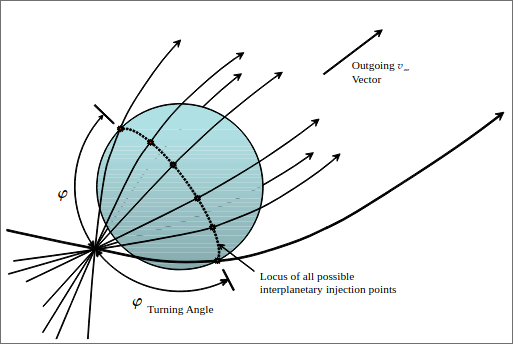
\includegraphics[width=\linewidth]{fig1.png}}
		\caption{Example Earth hyperbolic departure trajectories satisfying $v_{\infty}$. Image from Fundementals of Astrodynamics and Applications \cite{b4}}
		\label{fig}
	\end{figure}
	
	The hyperbolic periapsis velocity and circular velocity can be solved as follows:
	\[
	\prescript{I(body)}{}{v_{circ}} = \sqrt{\frac{\mu_{body}}{r_{p(body)}}}
	\quad\text{,}\quad
	\prescript{I(body)}{}{v_{hp}} = \sqrt{v_{\infty}^2 + \frac{2\mu_{body}}{r_{p(body)}}}
	\]
	Subsequently,
	\[
	\Delta v_{body} = |\prescript{I(body)}{}{v_{hp}} - \prescript{I(body)}{}{v_{circ}}|
	\]
	This gives the delta-v to reach a circular orbit of $r_{p(body)}$ at each body based on the transfer orbit velocity at that body. Additional information, such as the time to get from body1 to body2 and the about the TODO transfer can be found:
	\[
	t_{transfer} = \pi \sqrt{\frac{a_{transfer}^3}{\mu_0}}
	\quad\text{,}\quad
	TODO
	\]
	
	\subsection{Patched Conics Lambert Solution}
	Solving an interplanetary transfer using a lambert solution follows essentially the same process, with two exceptions: the positions of the planets at departure and arrival must be known (typically they are found by pre-determining the time of flight), and the velocities at body 1 and body 2 are given by the lambert solver. 
	
	\section{Results}
	
	\section{Conclusions and Future Work}
	
	\begin{thebibliography}{00}
		\bibitem{b1} G. D. Quinlan and S. Tremaine, "On the reliability of gravitational N-body integrations," Monthly Notices of the Royal Astronomical Society, vol. 259, no. 3, pp. 722-736, Dec. 1992, doi: 10.1093/mnras/259.3.722.
		\bibitem{b2} M. W. Weeks and S. W. Thrasher, "Comparison of Fixed and Variable Time Step Trajectory Integration Methods for Cislunar Trajectories," presented at the 17th AAS/AIAA Space Flight Mechanics Meeting, Sedona, AZ, USA, Jan. 28–Feb. 1, 2007.
		\bibitem{b3} J. R. Scott and M. C. Martini, "High Speed Solution of Spacecraft Trajectory Problems Using Taylor Series Integration," presented at the Astrodynamics Specialist Conference and Exhibit, Honolulu, HI, USA, Aug. 18–21, 2008.
		\bibitem{b4} D. A. Allado, Fundamentals of Astrodynamics and Applications. Microcosm Press, 2013.
		
	\end{thebibliography}
	
\end{document}
